\documentclass[final]{article}

\usepackage[utf8]{inputenc}
\usepackage[T1]{fontenc}
\usepackage[brazilian]{babel}
\usepackage{lmodern}
\usepackage[scaled=0.95]{helvet}
\renewcommand{\familydefault}{\sfdefault}

\usepackage[paperwidth=90cm, paperheight=120cm, margin=0cm]{geometry}
\usepackage{amsmath, amssymb, amsfonts}
\usepackage{booktabs}
\usepackage{array}
\usepackage{multicol}
\usepackage{graphicx}
\usepackage{xcolor}
\usepackage{tikz}
\usepackage{hyperref}

\definecolor{ufabcgreen}{HTML}{006633}
\definecolor{textdark}{HTML}{1A1A1A}

\hypersetup{
    colorlinks=true,
    urlcolor=ufabcgreen,
    linkcolor=ufabcgreen
}

\pagestyle{empty}
\setlength{\parindent}{0pt}
\setlength{\parskip}{0.45em}

% Destaque em verde institucional idêntico ao Exemplo 2
\newcommand{\destaque}[1]{\textcolor{ufabcgreen}{\textbf{#1}}}

% Títulos de seção no padrão Exemplo 2: 34pt, negrito, MAIÚSCULO, SEM NÚMERO
\newcommand{\postersection}[1]{%
    \par\vspace{0.6em}%
    {\fontsize{34}{40}\selectfont\bfseries #1}%
    \par\vspace{0.25em}%
}

% Legendas de figuras e tabelas idênticas ao Exemplo 2: 25pt
\newcommand{\postercaption}[2]{%
    \par\vspace{0.25em}%
    {\fontsize{25}{30}\selectfont\textbf{#1:} #2}%
    \par\vspace{0.35em}%
}

\begin{document}
\color{textdark}
\fontsize{29}{35}\selectfont

% ====================================================================
% PÔSTER EM PÁGINA ÚNICA (90cm x 120cm) COM TIKZ OVERLAY
% ====================================================================
\begin{tikzpicture}[remember picture, overlay, inner sep=0pt, outer sep=0pt]

    % ----------------------------------------------------------------
    % 1. CABEÇALHO NO TOPO (y = 0cm até y = -12cm)
    % ----------------------------------------------------------------
    % Caixa verde: margem de 5.25cm até 52.85cm (largura 47.6cm, altura 12cm)
    % Cantos inferiores arredondados com raio 4cm; cantos superiores retos
    \fill[ufabcgreen, rounded corners=4cm] (5.25cm, -12cm) rectangle (52.85cm, 0cm);
    \fill[ufabcgreen] (5.25cm, -4cm) rectangle (52.85cm, 0cm);

    % Título principal em branco, centralizado dentro da caixa verde
    \node[anchor=center, text=white, text width=45.5cm, align=center] at (29.05cm, -6.0cm) {
        {\fontsize{50}{58}\selectfont\bfseries
        PROBLEMAS DE FLUXOS EM REDES:\\[0.25em]
        TEORIA, ALGORITMOS E IMPLEMENTAÇÕES}
    };

    % Logos superiores ancoradas na base do cabeçalho (y = -12.0cm)
    % ufabc.png: largura 13cm (58.0cm a 71.0cm, centro em 64.5cm), altura 10.6cm
    \node[anchor=south] at (64.5cm, -12.0cm) {
        
\includegraphics[height=10.6cm]{poster/logos/ufabc.png}
    };
    % uscs.png: largura 13cm (73.5cm a 86.5cm, centro em 80.0cm), largura 12.6cm
    \node[anchor=south] at (80.0cm, -12.0cm) {
        
\includegraphics[width=12.6cm]{poster/logos/uscs.png}
    };

    % ----------------------------------------------------------------
    % 2. FAIXA DE AUTORES E AFILIAÇÃO (y = -12cm até y = -20.8cm, altura 8.8cm)
    % ----------------------------------------------------------------
    \node[anchor=north, text width=84.8cm, align=center] at (45.0cm, -12.8cm) {
        {\fontsize{34}{40}\selectfont\bfseries Gabriel Frigo, Cristiane Maria Sato}\\[0.3em]
        {\fontsize{29}{35}\selectfont
        Centro de Matemática, Computação e Cognição -- Universidade Federal do ABC\\[0.15em]
        Av. dos Estados, 5001 -- Bangú, Santo André - SP}\\[0.25em]
        {\fontsize{27}{33}\selectfont\ttfamily \{gabriel.frigo@aluno.ufabc.edu.br, cristiane.sato@ufabc.edu.br\}}
    };

    % ----------------------------------------------------------------
    % 3. RODAPÉ INFERIOR (y = -110.8cm até y = -120cm, altura 9.2cm)
    % ----------------------------------------------------------------
    % Área de Apoio (x = 0cm até 21.8cm, fundo branco)
    % Texto "Apoio:" com margem esquerda de 1.2cm
    \node[anchor=north west] at (1.2cm, -111.4cm) {
        {\fontsize{30}{36}\selectfont\bfseries Apoio:}
    };

    % Logos do Apoio:
    % Linha 1: ufabc.png (height 3.4cm) e uscs.png (width 4.3cm)
    \node[anchor=south] at (2.95cm, -116.3cm) {
        
\includegraphics[height=3.4cm]{poster/logos/ufabc.png}
    };
    \node[anchor=south] at (7.35cm, -116.3cm) {
        
\includegraphics[width=4.3cm]{poster/logos/uscs.png}
    };

    % Linha 2: cnpq.png (height 2.1cm) centrada abaixo de ufabc e uscs
    \node[anchor=south] at (5.15cm, -119.2cm) {
        
\includegraphics[height=2.1cm]{poster/logos/cnpq.png}
    };

    % Coluna 3: toca.png (largura 10.8cm) ocupando as duas linhas
    \node[anchor=center] at (15.7cm, -115.8cm) {
        
\includegraphics[width=10.8cm]{poster/logos/toca.png}
    };

    % Bloco verde direito do rodapé (x = 21.8cm a 90cm, y = -120cm a -110.8cm)
    % Contido estritamente com clip para eliminar qualquer vazamento
    \begin{scope}
        \clip (21.8cm, -120cm) rectangle (90cm, -110.8cm);
        \fill[ufabcgreen] (21.8cm, -120cm) rectangle (90cm, -110.8cm);
        \node[anchor=south east, opacity=0.3] at (90cm, -120cm) {
            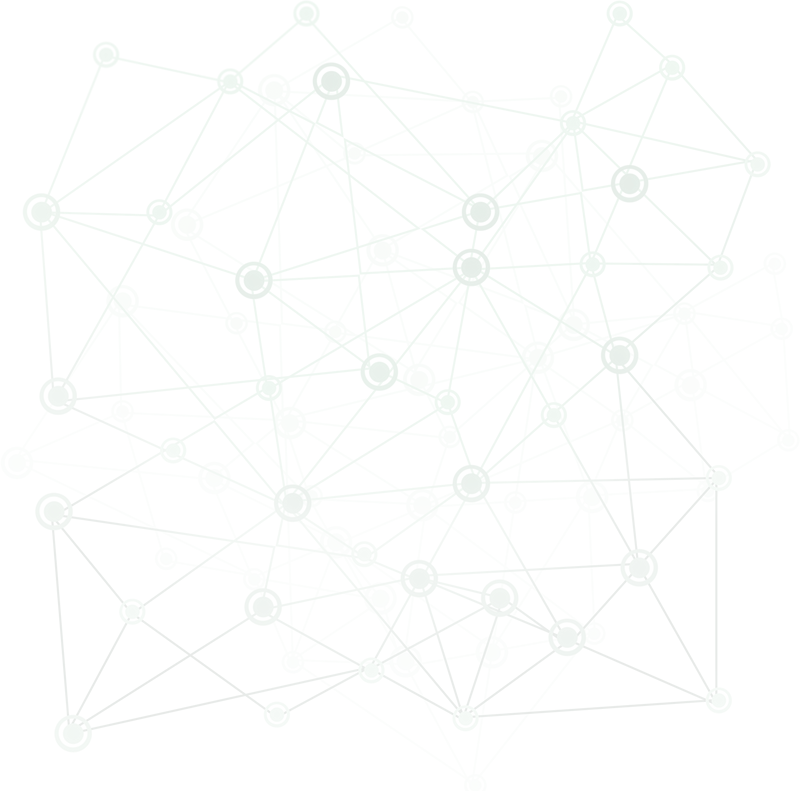
\includegraphics[width=42cm]{poster/logos/background.png}
        };
    \end{scope}

    % Texto institucional do evento 2026 (alinhado à direita com inset de 1.5cm)
    \node[anchor=east, align=right, inner sep=0pt] at (88.5cm, -115.4cm) {
        {\fontsize{72}{82}\selectfont\bfseries\color{white}\mbox{XVI Encontro de Iniciação Científica}}\\[0.2em]
        {\fontsize{32}{38}\selectfont\bfseries\color{white}\mbox{XIX Simpósio de Iniciação Científica da UFABC}}\\[0.15em]
        {\fontsize{32}{38}\selectfont\bfseries\color{white}\mbox{21º Congresso de Iniciação Científica da USCS}}
    };

\end{tikzpicture}

% ====================================================================
% CORPO CENTRAL (Área útil: x = 2.6cm a 87.4cm, y = -20.8cm a -109.3cm)
% ====================================================================
\vspace*{20.8cm}
\noindent
\hspace{2.6cm}\begin{minipage}[t]{84.8cm}
\setlength{\columnsep}{2.5cm}
\begin{multicols}{2}

% --------------------------------------------------------------------
\postersection{INTRODUÇÃO}
% --------------------------------------------------------------------
Os problemas de \destaque{Fluxo Máximo (MF)} e \destaque{Fluxo de Custo Mínimo (MCF)} constituem modelos fundamentais da Otimização Combinatória e da Teoria dos Grafos. Em uma rede capacitada $G = (V, A)$, busca-se uma função de fluxo $f: A \to \mathbb{R}_+$ que respeite restrições de capacidade ($0 \le f(u,v) \le c(u,v)$) e conservação de fluxo em todos os vértices intermediários.

\vspace{0.3em}
\begin{center}
\fboxrule=0.12em
\fboxsep=0.7em
\fbox{%
\begin{minipage}{0.95\linewidth}
    \textcolor{ufabcgreen}{\textbf{Problema:}} \textbf{Fluxo de Custo Mínimo (MCF)}\\
    \textbf{Entrada:} Rede $G=(V, A)$, capacidades $c(u,v)$, custos $w(u,v)$, fonte $s$ e sorvedouro $t$.\\
    \textbf{Saída:} Fluxo viável $f$ de valor $|f|$ máximo que minimiza o custo total $\sum_{a \in A} w(a) f(a)$.
\end{minipage}%
}
\end{center}
\vspace{0.3em}

\textbf{Objetivos centrais da pesquisa:}
\begin{itemize}
    \item \textbf{Rigor Teórico:} Demonstração axiomática dos teoremas de dualidade, cortes e otimalidade primal-dual.
    \item \textbf{Engenharia em C++23:} Motores algorítmicos orientados a objetos de alta performance sem dependências externas.
    \item \textbf{Modelagem e Aplicações:} Reduções polinomiais clássicas e segmentação interativa de imagens via corte mínimo.
    \item \textbf{Validação Empírica:} Avaliação experimental sistemática no benchmark canônico DIMACS.
\end{itemize}

% --------------------------------------------------------------------
\postersection{FUNDAMENTAÇÃO TEÓRICA E DUALIDADE}
% --------------------------------------------------------------------
\textbf{Teorema do Fluxo Máximo e Corte Mínimo (Ford-Fulkerson, 1956):}
Em toda rede $G = (V, A, c, s, t)$, para um fluxo viável $f$, são equivalentes:
\begin{enumerate}
    \item $f$ possui valor $|f|$ máximo na rede;
    \item A rede residual $G_f$ não admite caminhos aumentantes de $s$ a $t$;
    \item Existe um corte $(S, T)$ com $s \in S, t \in T$ tal que $|f| = c(S, T)$.
\end{enumerate}

\textbf{Teorema da Integralidade e Aplicações:}
Se as capacidades $c(u,v)$ são inteiras, existe fluxo máximo integral $f^*$, viabilizando reduções aos teoremas de \textbf{Menger}, \textbf{König} e \textbf{Hall}.

\textbf{Dualidade Linear e Potenciais de Vértice:}
Pela total unimodularidade da matriz de incidência, um fluxo viável $f$ é de custo mínimo se, e somente se, existem potenciais $\pi: V \to \mathbb{R}$ tais que o \destaque{custo reduzido} satisfaz:
\[
c^\pi(u, v) = w(u, v) + \pi(u) - \pi(v) \ge 0 \quad \forall (u, v) \in A_f.
\]

% --------------------------------------------------------------------
\postersection{ARQUITETURA E MOTORES ALGORÍTMICOS}
% --------------------------------------------------------------------
As classes \texttt{FlowNetwork} e \texttt{CostNetwork} em C++23 armazenam os arcos em vetores contíguos \texttt{std::vector<Edge>}. O arco reverso é acessado em $\mathcal{O}(1)$ via \texttt{edge\_id \^{} 1}, otimizando a localidade de referência em cache L1/L2.

\vspace{0.25cm}
\begin{center}
{\fontsize{22}{27}\selectfont
\renewcommand{\arraystretch}{1.18}
\begin{tabular}{lllr}
\toprule
\textbf{Domínio} & \textbf{Classe C++23} & \textbf{Estratégia} & \textbf{Complexidade} \\
\midrule
\textbf{Fluxo} & \texttt{FordFulkerson} & Busca em profundidade (DFS) & $\mathcal{O}(|A| \cdot |f^*|)$ \\
\textbf{Máximo} & \texttt{EdmondsKarp} & Caminhos mínimos (BFS) & $\mathcal{O}(|V| \cdot |A|^2)$ \\
\textbf{(MF)} & \texttt{Dinic} & Grafo em níveis + bloqueante & $\mathcal{O}(|V|^2 \cdot |A|)$ \\
 & \texttt{PushRelabel} & Pré-fluxo com fila FIFO & $\mathcal{O}(|V|^3)$ \\
 & \texttt{PushRelabelImproved} & \textit{Highest-Label} + \textit{Gap} & $\mathcal{O}(|V|^2 \sqrt{|A|})$ \\
\midrule
\textbf{Custo} & \texttt{CycleCanceling} & Cancelamento de ciclos & $\mathcal{O}(|V| \cdot |A|^2 C U)$ \\
\textbf{Mínimo} & \texttt{SuccessiveShortest} & Caminhos sucessivos (SPFA) & $\mathcal{O}(|V| \cdot |A| \cdot |f^*|)$ \\
\textbf{(MCF)} & \texttt{SuccessiveShortestDijkstra} & Potenciais + Dijkstra & $\mathcal{O}(|f^*| |A| \log |V|)$ \\
 & \texttt{NetworkSimplex} & Árvore geradora (\texttt{thread}) & Polinomial \\
\bottomrule
\end{tabular}
}
\end{center}
\postercaption{Tabela 1}{Motores exatos implementados em C++23 e complexidades teóricas.}

% --------------------------------------------------------------------
\postersection{SEGMENTAÇÃO DE IMAGENS VIA CORTE MÍNIMO}
% --------------------------------------------------------------------
Seguindo Boykov e Jolly (2001), a imagem é formulada como um digrafo $V = \mathcal{P} \cup \{s, t\}$. Sementes interativas de objeto ($\mathcal{O}$) e fundo ($\mathcal{B}$) definem \textit{t-links} com capacidade infinita ($\infty$), enquanto vizinhos 4-conexos definem \textit{n-links} ponderados pelo gradiente RGB:
\[
c(p, q) = \operatorname{round}\!\left(K_0 \cdot \exp\!\left(-\frac{\|I(p) - I(q)\|_2^2}{2\sigma^2}\right)\right) + 1.
\]

\vspace{0.2cm}
\begin{center}
{\fontsize{22}{27}\selectfont
\renewcommand{\arraystretch}{1.12}
\setlength{\tabcolsep}{6pt}
\begin{tabular}{cccc}
\toprule
\textbf{Amostra} & \textbf{Original} & \textbf{Sementes} & \textbf{Corte Mínimo $(S, T)$} \\
\midrule
\texttt{duck} &

\includegraphics[height=3.4cm]{poster/imagens/duck_orig.png} &

\includegraphics[height=3.4cm]{poster/imagens/duck_seeds.png} &

\includegraphics[height=3.4cm]{poster/imagens/duck_seg.png} \\
\texttt{ducks} &

\includegraphics[height=3.4cm]{poster/imagens/ducks_orig.png} &

\includegraphics[height=3.4cm]{poster/imagens/ducks_seeds.png} &

\includegraphics[height=3.4cm]{poster/imagens/ducks_seg.png} \\
\texttt{balloons} &
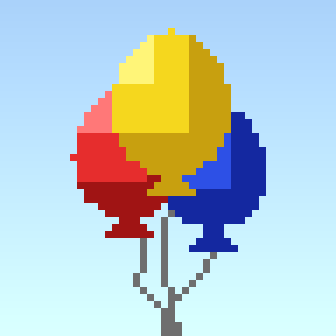
\includegraphics[height=3.4cm]{poster/imagens/balloons_orig.png} &

\includegraphics[height=3.4cm]{poster/imagens/balloons_seeds.png} &

\includegraphics[height=3.4cm]{poster/imagens/balloons_seg.png} \\
\texttt{circle} &

\includegraphics[height=3.4cm]{poster/imagens/circle_orig.png} &

\includegraphics[height=3.4cm]{poster/imagens/circle_seeds.png} &

\includegraphics[height=3.4cm]{poster/imagens/circle_seg.png} \\
\bottomrule
\end{tabular}
}
\end{center}
\postercaption{Figura 1}{Segmentação interativa exata via partição de corte mínimo $s$-$t$.}

\columnbreak

% --------------------------------------------------------------------
\postersection{RESULTADOS EXPERIMENTAIS (DIMACS)}
% --------------------------------------------------------------------
Avaliação de desempenho em \textbf{80 instâncias canônicas do 1st DIMACS Implementation Challenge} (famílias \textit{wash}, \textit{genrmf} e \textit{netgen}), compiladas com otimização \texttt{g++ -O2}.

\vspace{0.2cm}
\begin{center}
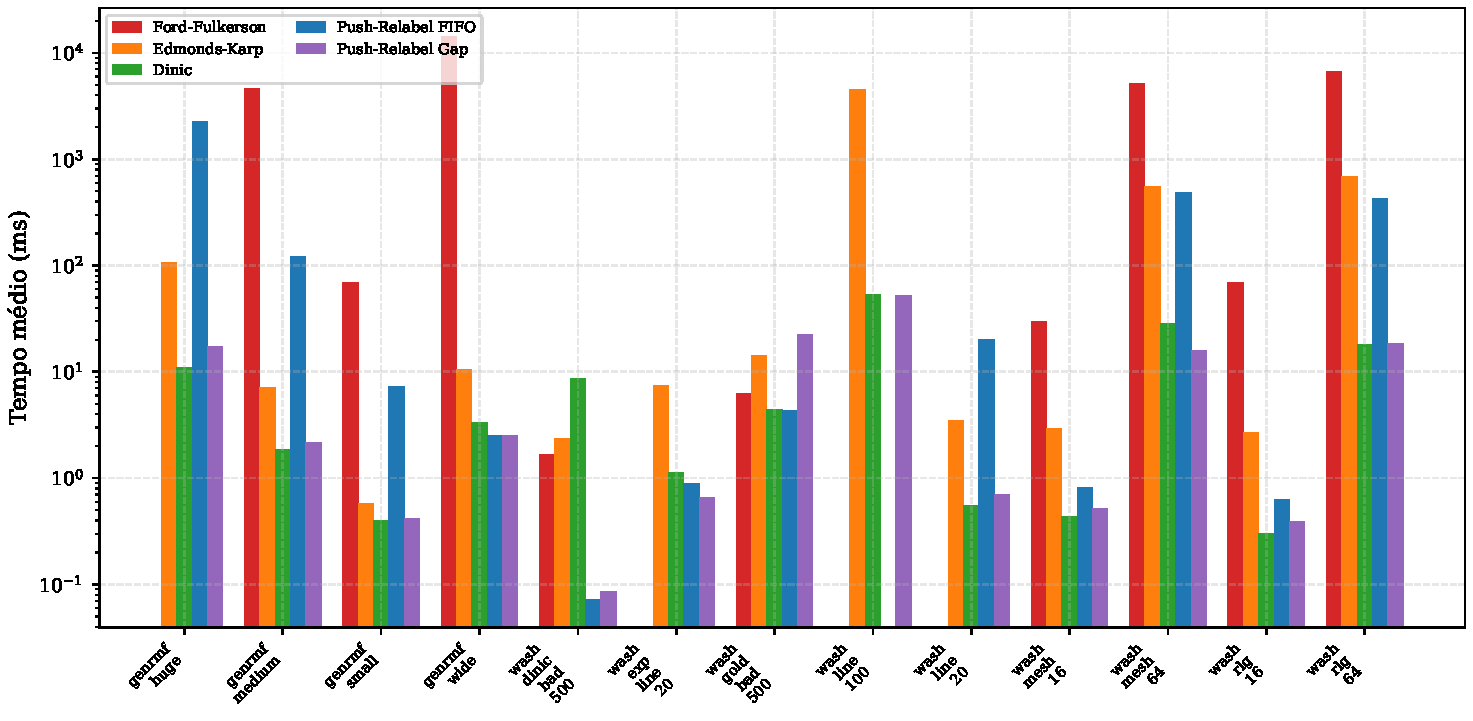
\includegraphics[width=0.485\linewidth]{figuras/ic/bars_maxflow.pdf}\hfill
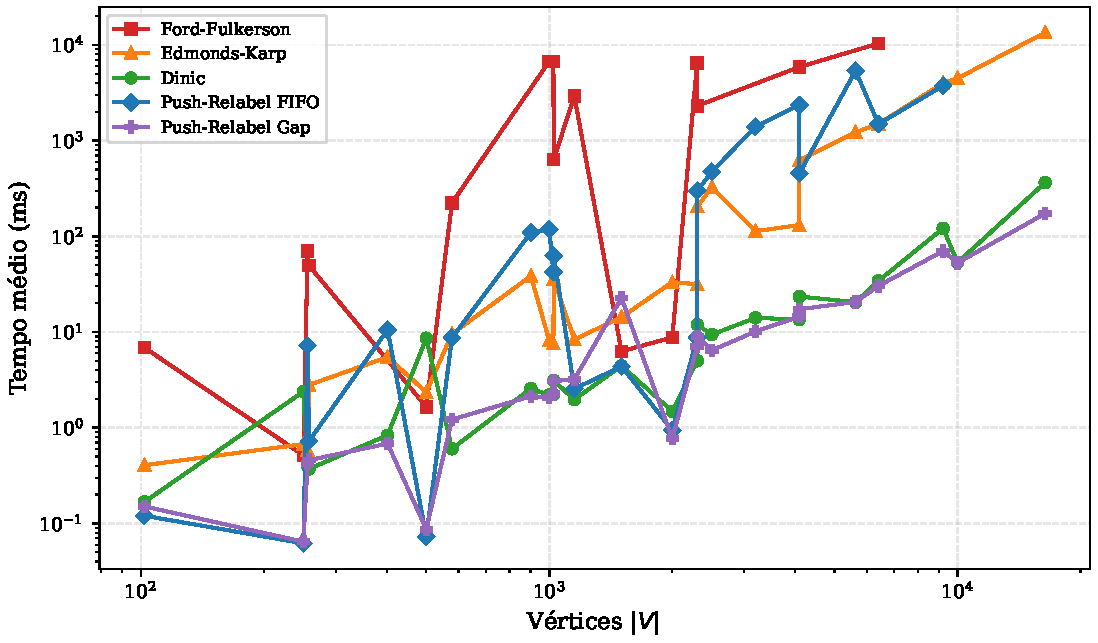
\includegraphics[width=0.485\linewidth]{figuras/ic/scalability_maxflow.pdf}\\[0.3cm]
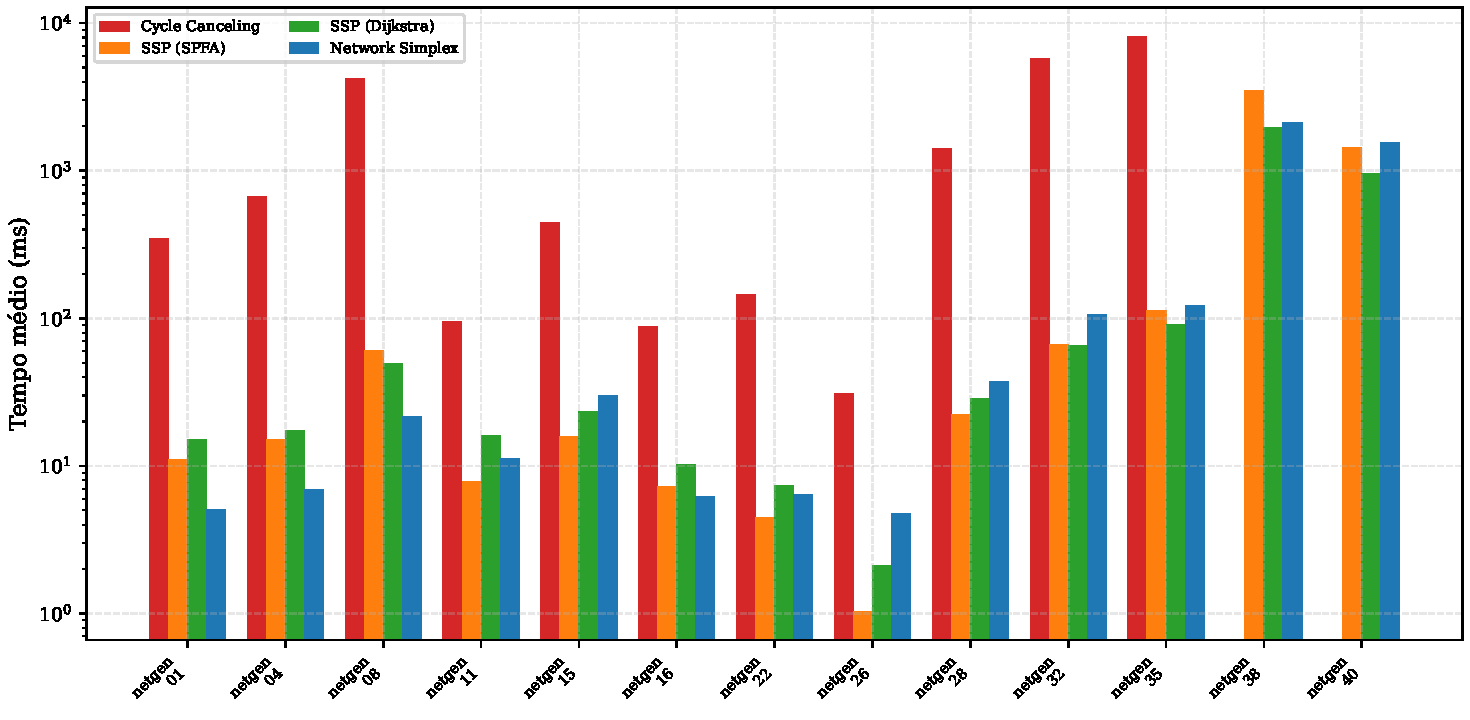
\includegraphics[width=0.485\linewidth]{figuras/ic/bars_mincost.pdf}\hfill
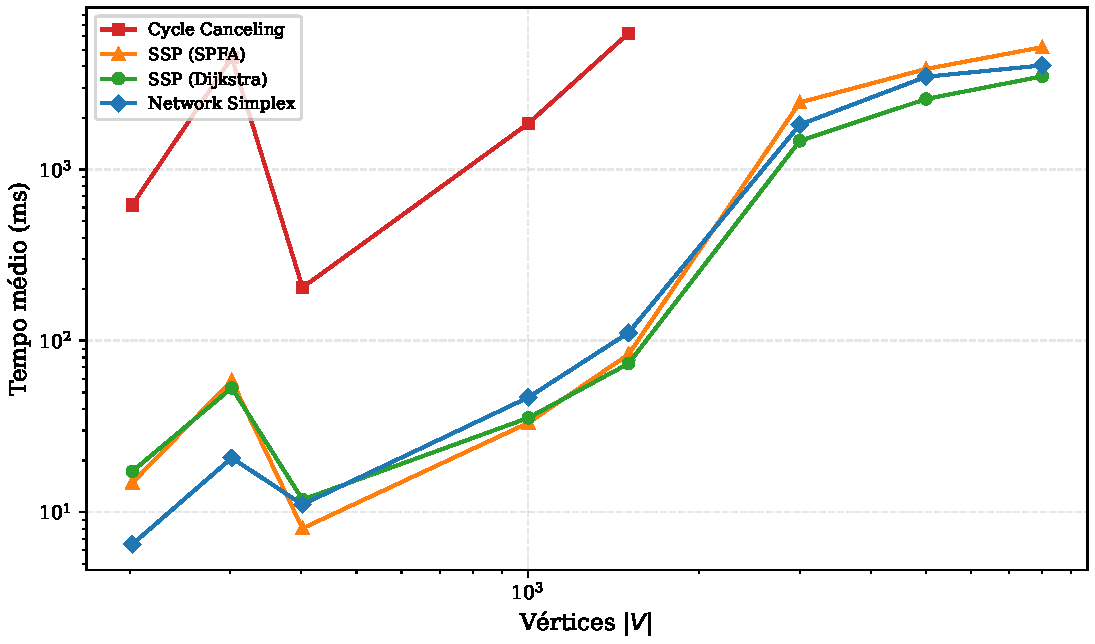
\includegraphics[width=0.485\linewidth]{figuras/ic/scalability_mincost.pdf}
\end{center}
\postercaption{Figura 2}{Tempo de CPU (ms) e escalabilidade em instâncias DIMACS.}

\vspace{0.2cm}
\begin{center}
{\fontsize{20}{25}\selectfont
\renewcommand{\arraystretch}{1.15}
\setlength{\tabcolsep}{5.5pt}
\begin{tabular}{lrrr|rrrrr}
\toprule
\textbf{Instância (MF)} & $|V|$ & $|A|$ & $f^*$ & \textbf{FF} & \textbf{EK} & \textbf{Dinic} & \textbf{PR} & \textbf{PR-Gap} \\
\midrule
\texttt{wash\_mesh\_64} & 4.098 & 12.224 & 105.788 & 23,5 & 25,6 & \textbf{1,53} & 18,3 & 2,84 \\
\texttt{wash\_rlg\_64} & 4.098 & 12.160 & 29.749 & 16,6 & 28,2 & 2,36 & 27,8 & \textbf{1,96} \\
\texttt{genrmf\_huge} & 4.096 & 18.368 & 134.538 & TLE & 106 & \textbf{11,0} & 2.261 & 12,1 \\
\bottomrule
\end{tabular}

\vspace{0.25cm}
\begin{tabular}{lrrrr|rrrr}
\toprule
\textbf{Instância (MCF)} & $|V|$ & $|A|$ & $f^*$ & $z^*$ & \textbf{CC} & \textbf{SSP-SPFA} & \textbf{SSP-Dijk} & \textbf{Simplex} \\
\midrule
\texttt{netgen\_08} & 402 & 3.005 & 200k & 325.1M & 1.560 & 50,0 & 52,0 & \textbf{18,5} \\
\texttt{netgen\_15} & 402 & 4.560 & 4.000 & 4.49M & 536 & 25,4 & \textbf{11,5} & 17,9 \\
\texttt{netgen\_40} & 3.002 & 22.800 & 200k & 266.2M & TLE & 1.448 & 1.240 & \textbf{737} \\
\bottomrule
\end{tabular}
}
\end{center}
\postercaption{Tabela 2}{Tempo de CPU (ms) nas principais instâncias do benchmark DIMACS.}

\textbf{Análise dos resultados experimentais:}
\begin{itemize}
    \item Em Fluxo Máximo, \texttt{PushRelabelImproved} e \texttt{Dinic} superam métodos elementares em até duas ordens de grandeza em redes densas e gargalos adversariais.
    \item Em Custo Mínimo, o \texttt{NetworkSimplex} demonstra desempenho superior consistente, com tempo de execução até $2\times$ menor que o algoritmo de caminhos sucessivos.
\end{itemize}

% --------------------------------------------------------------------
\postersection{AGRADECIMENTOS}
% --------------------------------------------------------------------
Este trabalho foi financiado pelo Conselho Nacional de Desenvolvimento Científico e Tecnológico (CNPq), processo PIBIC 143763/2024-5.
Agradecimentos à Profa.\ Dra.\ Cristiane Maria Sato pela orientação, e à Universidade Federal do ABC (UFABC).

\destaque{Código-fonte e documentação:} \url{https://github.com/Gabrielfrigo4/Network-Flow}

% --------------------------------------------------------------------
\postersection{BIBLIOGRAFIA}
% --------------------------------------------------------------------
{\fontsize{26}{32}\selectfont
\begin{itemize}
    \setlength{\itemsep}{0.25em}
    \item[{[1]}] AHUJA, R.\ K.; MAGNANTI, T.\ L.; ORLIN, J.\ B. \textit{Network Flows: Theory, Algorithms, and Applications}. Prentice Hall, 1993.
    \item[{[2]}] BOYKOV, Y.\ Y.; JOLLY, M.-P. Interactive graph cuts for optimal boundary and region segmentation of objects in N-D images. In: \textit{Proc.\ IEEE ICCV}, 2001.
    \item[{[3]}] DINIC, E.\ A. Algorithm for solution of a problem of maximum flow in a network with power estimation. \textit{Soviet Math.\ Doklady}, 1970.
    \item[{[4]}] FORD, L.\ R.; FULKERSON, D.\ R. Maximal flow through a network. \textit{Canadian Journal of Mathematics}, v. 8, p. 399--404, 1956.
\end{itemize}
}

\end{multicols}
\end{minipage}

\end{document}
